\documentclass[11pt,a4paper]{article}

\usepackage[margin=1in]{geometry}
\usepackage[T1]{fontenc}
\usepackage[utf8]{inputenc}
\usepackage{lmodern}
\usepackage{microtype}
\usepackage{amsmath,amssymb}
\usepackage{booktabs}
\usepackage{graphicx}
\usepackage{array}
\usepackage{tabularx}
\usepackage{longtable}
\usepackage{multirow}
\usepackage{xcolor}
\usepackage{hyperref}
\usepackage{xurl}
\usepackage{enumitem}
\usepackage{caption}
\usepackage{subcaption}
\usepackage{fancyhdr}
\usepackage{lastpage}

\hypersetup{hidelinks}
\graphicspath{{figures/primary_robustness_20260813/}}
\captionsetup{font=small,labelfont=bf}
\setlist{nosep,leftmargin=*}
\setlength{\parindent}{1.5em}
\setlength{\parskip}{0.25em}
\setlength{\emergencystretch}{2em}
\renewcommand{\arraystretch}{1.15}

\pagestyle{fancy}
\fancyhf{}
\fancyhead[L]{\small Primary LLM-DNA Robustness Experiment}
\fancyhead[R]{\small Weekly Progress Update}
\fancyfoot[C]{\small \thepage\ of \pageref{LastPage}}
\renewcommand{\headrulewidth}{0.4pt}
\renewcommand{\footrulewidth}{0pt}

\newcommand{\code}[1]{\texttt{\detokenize{#1}}}
\newcommand{\interim}{\textcolor{gray}{\textit{Interim}}}

\title{Primary LLM-DNA Robustness Experiment\\
\large Weekly Progress Update: Recovery, Decoding Surface, and DistDNA Pilot}
\author{}
\date{Updated August 13, 2026}

\begin{document}
\maketitle

\begin{abstract}
This report records progress since the frozen August 5 report. It does not
repeat the full experimental protocol or previously defined formulas. A
failure-specific recovery pass increased the validated primary grid from
2,528 to 2,553 successful artifacts out of 2,600 and increased the strict
all-run cohort from 59 to 69 models. Using this fixed 69-model cohort, we add
an interim analysis of the joint temperature and top-$p$ surface. Exact-model
Top-1 retrieval against a deterministic $T=0$ gallery declines sharply as
temperature increases, while the observed top-$p$ effect is smaller and
conditional on temperature. We also specify a leakage-free, matched-budget
four-seed pilot for DistDNA. All accuracy estimates remain interim because
recovery is running and the strict cohort is below the preregistered minimum
of 80 models.
\end{abstract}

\section{Progress since August 5}

The original August 5 report remains frozen. Table~\ref{tab:weekly-progress}
contains only changes observed by the August 13 live snapshot.

\begin{table}[htbp]
\centering
\caption{Primary-grid progress from August 5 to the August 13 live snapshot.}
\label{tab:weekly-progress}
\begin{tabular}{lrrr}
\toprule
Measure & August 5 & August 13 & Change \\
\midrule
Successful artifacts & 2,528/2,600 & 2,553/2,600 & $+25$ \\
Artifact coverage & 97.2\% & 98.2\% & $+1.0$ pp \\
Slots without success & 72 & 47 & $-25$ \\
Strict all-26-run cohort & 59/100 & 69/100 & $+10$ \\
Explicit-seed successes & 572 & 597 & $+25$ \\
Historical unknown-seed only & 1,956 & 1,956 & no change \\
\bottomrule
\end{tabular}
\end{table}

Figure~\ref{fig:live-grid} separates artifact coverage from seed provenance.
The recovery pass writes successful results alongside the historical data and
does not overwrite prior artifacts. At the figure timestamp, the largest
remaining gap was $T=0.5,p=1.0$, with 176 of 200 planned artifacts successful.

\begin{figure}[htbp]
\centering
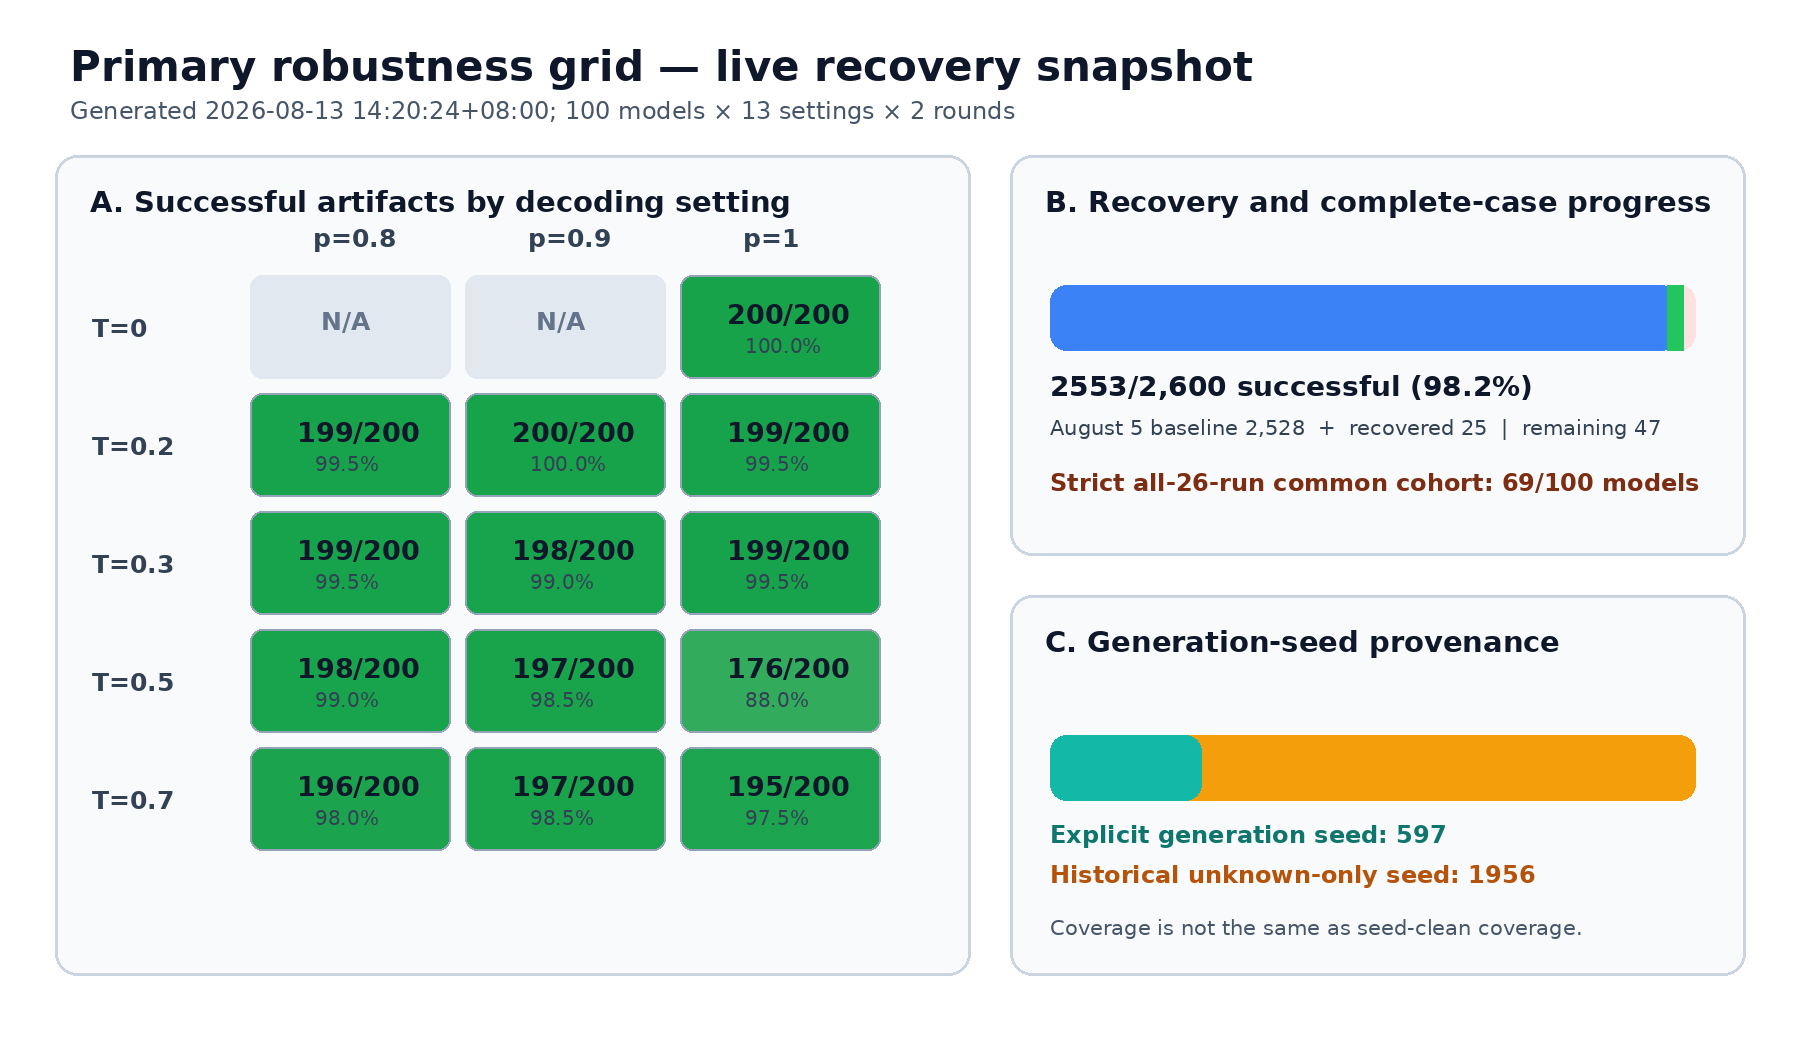
\includegraphics[width=\textwidth]{live_grid_seed_recovery.png}
\caption{Live primary-grid recovery snapshot. Panel A gives successful
artifact counts by decoding setting; Panel B reports overall and strict-cohort
progress; Panel C distinguishes explicit response-generation seeds from
historical artifacts whose generation seed is unknown. This is a timestamped
snapshot rather than a final result.}
\label{fig:live-grid}
\end{figure}

The recovery process was still active when this report was compiled. At the
Figure~\ref{fig:live-grid} timestamp it was running $T=0.5,p=0.9$, repeat 2,
with response-generation seed 42. The general recovery rule is 42 for
both $T=0.5$ rounds, and otherwise 42001 for repeat 1 and 42002 for repeat 2.

\section{Interim temperature and top-$p$ surface}
\label{sec:surface}

\subsection{Analysis definition}

The surface analysis uses the 69 models that have a successful artifact in
every one of the 26 planned run keys. Holding the cohort fixed makes all cells
directly comparable. For duplicate successful artifacts, selection prefers an
explicit seed 42001 or 42002, then another explicit seed, then an historical
unknown-seed artifact.

Two complementary comparisons are reported:

\begin{enumerate}
  \item \textbf{Fixed deterministic gallery.} The $T=0$, repeat-1 DNA vectors
        form the gallery. Each stochastic repeat-2 cell is queried against
        that same gallery. This is the primary visualization of decoding
        robustness.
  \item \textbf{Same-setting repeat stability.} For each $(T,p)$ cell,
        repeat 1 forms the gallery and repeat 2 forms the query. This measures
        reproducibility within a setting and should not be confused with a
        fixed-reference robustness test.
\end{enumerate}

Both comparisons use ordinary cosine retrieval and exact-model Top-1 as the
primary metric. Figure~\ref{fig:decoding-surface} reports the resulting curves
and grids.

\begin{figure}[p]
\centering
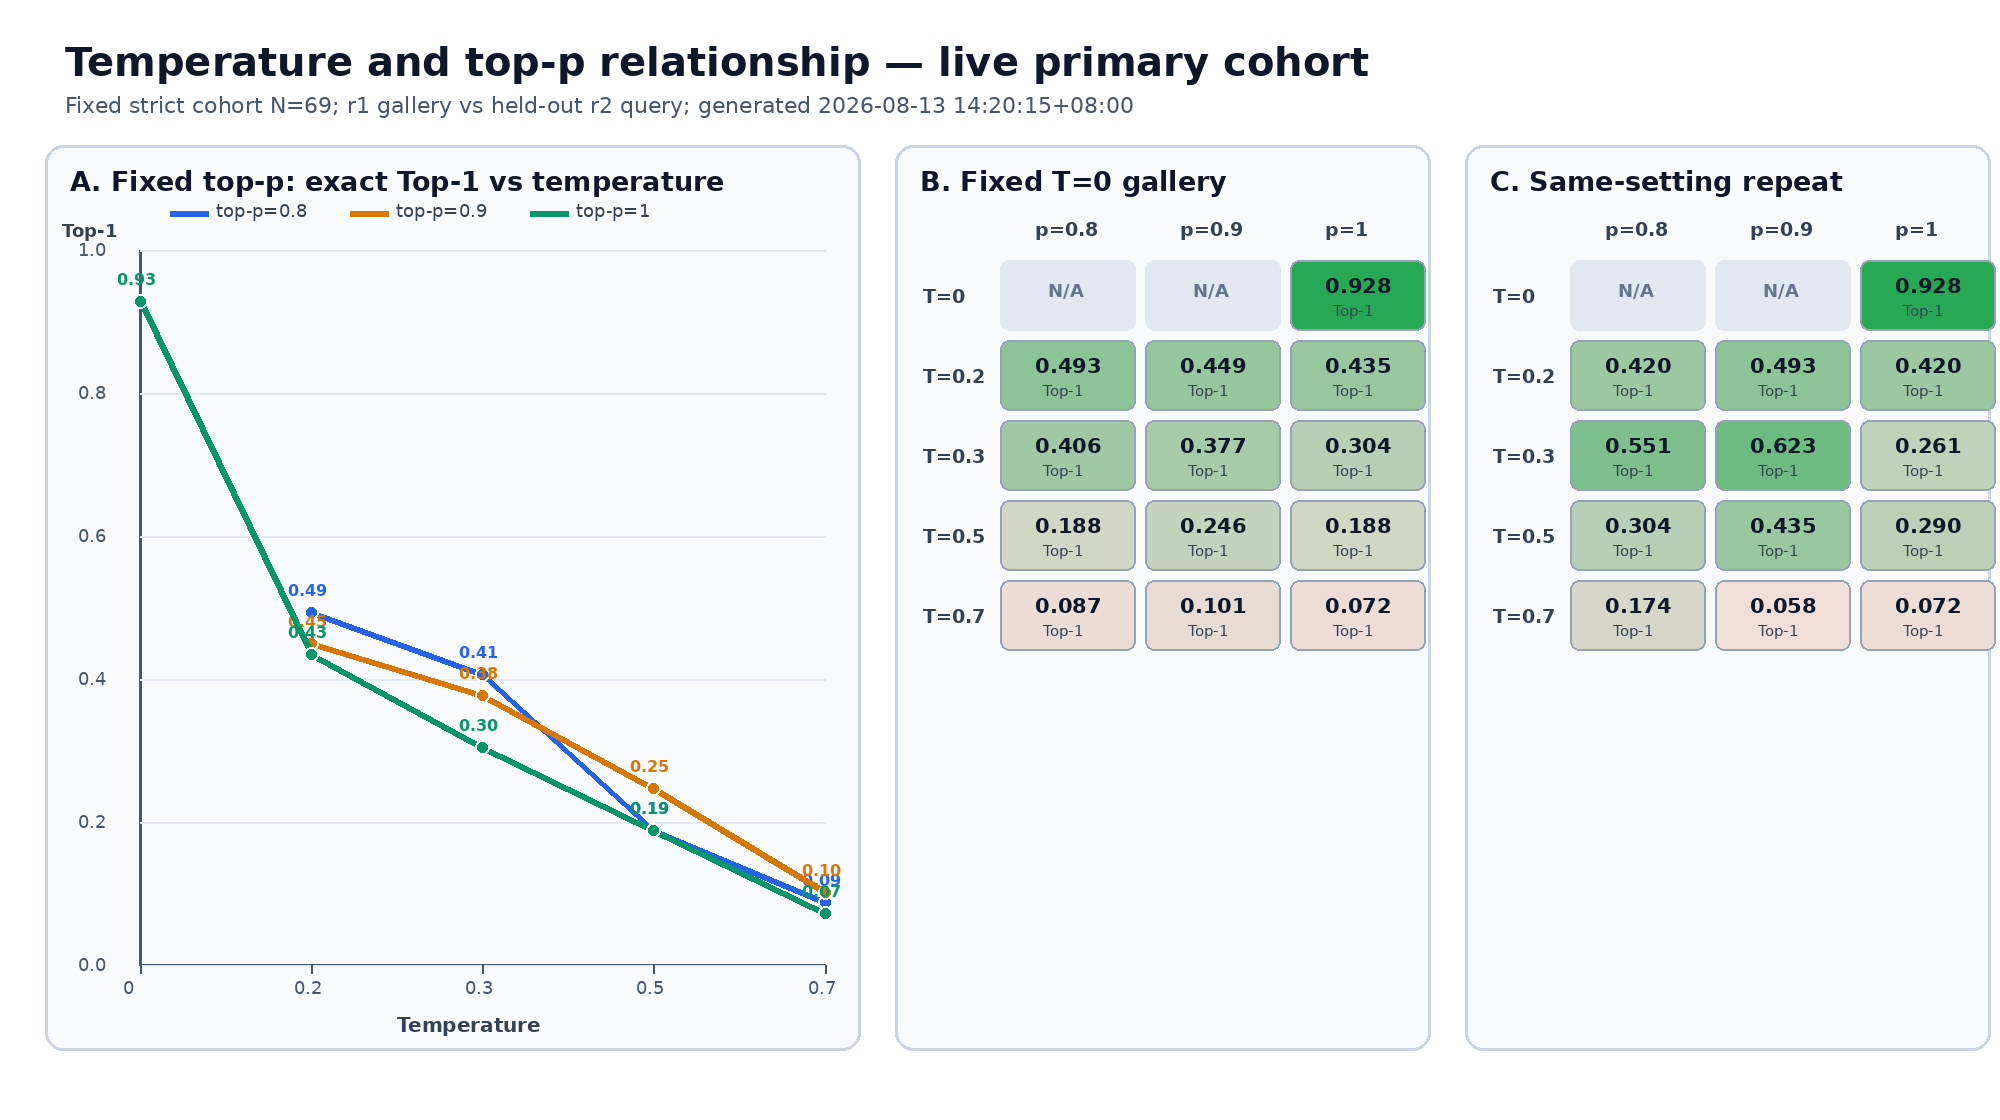
\includegraphics[width=\textwidth]{temperature_top_p_relationship.png}
\caption{Interim temperature--top-$p$ relationship on the fixed 69-model
strict cohort. Panel A fixes top-$p$ and traces exact-model Top-1 as temperature
changes. Panel B uses one deterministic $T=0$ reference gallery for every
query cell. Panel C instead uses the matching repeat-1 gallery for each cell.
All queries use held-out repeat 2.}
\label{fig:decoding-surface}
\end{figure}

\subsection{Observed pattern}

Table~\ref{tab:fixed-gallery-results} gives the fixed-gallery Top-1 values.
The dominant pattern is a strong temperature effect. At each top-$p$, accuracy
falls as temperature increases from 0.2 to 0.7. Top-$p$ changes the level of
the curve, but its ordering is not constant across temperatures.

\begin{table}[htbp]
\centering
\caption{Exact-model Top-1 against the fixed $T=0$ gallery ($N=69$).}
\label{tab:fixed-gallery-results}
\begin{tabular}{crrr}
\toprule
Temperature & $p=0.8$ & $p=0.9$ & $p=1.0$ \\
\midrule
$0$   & --    & --    & 0.928 \\
$0.2$ & 0.493 & 0.449 & 0.435 \\
$0.3$ & 0.406 & 0.377 & 0.304 \\
$0.5$ & 0.188 & 0.246 & 0.188 \\
$0.7$ & 0.087 & 0.101 & 0.072 \\
\bottomrule
\end{tabular}
\end{table}

Three descriptive observations follow.

\begin{itemize}
  \item Increasing temperature is associated with the largest accuracy loss.
        At $p=1.0$, Top-1 declines from 0.435 at $T=0.2$ to 0.072 at $T=0.7$.
  \item Lower top-$p$ is beneficial at $T=0.2$ and $T=0.3$, but the pattern
        is not monotone at $T=0.5$ or $T=0.7$. For example, $p=0.9$ is best
        at both of those temperatures.
  \item The changing top-$p$ ordering is suggestive of a temperature--top-$p$
        interaction, but it is not yet a formal interaction test. The final
        analysis should attach paired model-level uncertainty after recovery.
\end{itemize}

The same-setting panel is also non-monotone. It is stronger than the fixed
gallery at some cells, such as $(T,p)=(0.3,0.9)$, but remains weak at $T=0.7$.
This indicates that high stochasticity affects both cross-setting robustness
and within-setting repeatability.

\section{Bounded and jointly bounded decoding conditions}

The planned deployment analysis assumes that the exact decoding setting is
hidden but an upper temperature bound $T\leq\tau$ may be known. We extend that
view descriptively to a joint bound $T\leq\tau$ and $p\leq\pi$.

For every $(\tau,\pi)$ pair, the gallery is the per-model centroid across all
eligible repeat-1 cells. The deterministic control is always included because
top-$p$ is inactive at $T=0$. Repeat-2 cells supply the queries. Each decoding
cell receives equal weight. Figure~\ref{fig:bounded-surface} shows equal-cell
mean Top-1, worst-setting Top-1, and the joint mean grid.

\begin{figure}[p]
\centering
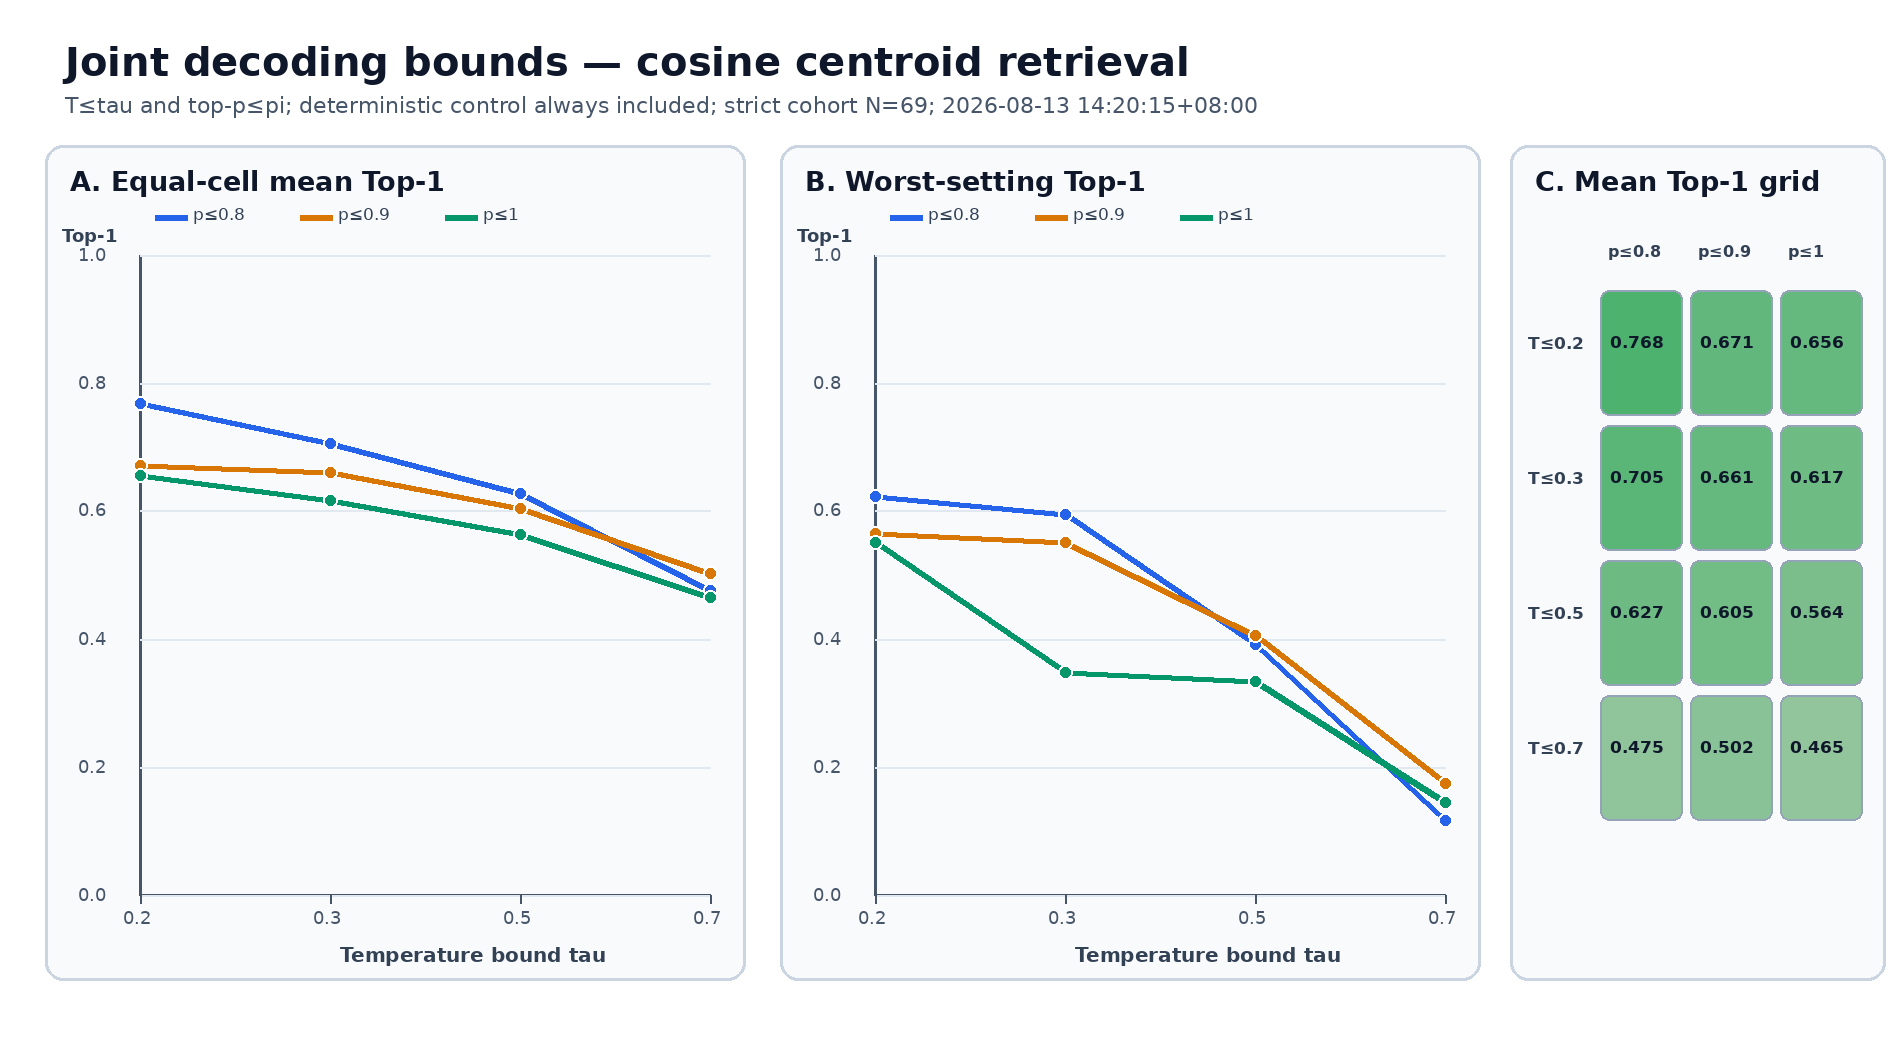
\includegraphics[width=\textwidth]{bounded_decoding_relationship.png}
\caption{Interim cosine-centroid performance under joint bounds
$T\leq\tau$ and $p\leq\pi$ on the fixed 69-model cohort. Panel A reports the
equal-cell mean; Panel B reports the worst eligible setting; Panel C shows the
mean surface. The deterministic control is included at every bound.}
\label{fig:bounded-surface}
\end{figure}

\begin{table}[htbp]
\centering
\caption{Equal-cell mean Top-1 under joint temperature and top-$p$ bounds.}
\label{tab:bounded-results}
\begin{tabular}{crrr}
\toprule
Temperature bound & $p\leq0.8$ & $p\leq0.9$ & $p\leq1.0$ \\
\midrule
$\tau=0.2$ & 0.768 & 0.671 & 0.656 \\
$\tau=0.3$ & 0.705 & 0.661 & 0.617 \\
$\tau=0.5$ & 0.627 & 0.605 & 0.564 \\
$\tau=0.7$ & 0.475 & 0.502 & 0.465 \\
\bottomrule
\end{tabular}
\end{table}

The bounded results reinforce the temperature trend. With $p\leq0.8$, mean
Top-1 declines from 0.768 at $\tau=0.2$ to 0.475 at $\tau=0.7$. The
worst-setting value declines more sharply, from 0.623 to 0.116. Restricting
top-$p$ improves the mean for $\tau\leq0.5$, but not monotonically at
$\tau=0.7$, where the $p\leq0.9$ mean is 0.502. Because the gallery centroid
and eligible query mixture both change with the bound, these comparisons are
deployment summaries rather than a causal decomposition of temperature and
top-$p$.

\section{Seed provenance and the four-seed extension}

Artifact coverage and seed-clean coverage must remain separate. Table
\ref{tab:seed-policy} records which existing artifacts can be reused in a
four-seed DistDNA study.

\begin{table}[htbp]
\centering
\caption{Response-generation seed policy.}
\label{tab:seed-policy}
\begin{tabularx}{\textwidth}{>{\raggedright\arraybackslash}p{0.25\textwidth}>{\raggedright\arraybackslash}p{0.20\textwidth}>{\raggedright\arraybackslash}X}
\toprule
Source & Recorded seed & Four-seed use \\
\midrule
$T\in\{0.2,0.3,0.7\}$ backfills & r1: 42001; r2: 42002 & Reusable when the exact model, setting, prompts, token budget, and seed match. \\
$T=0.5$ control/recovery & r1: 42; r2: 42 & Retain for the original grid, but regenerate for seed-clean evidence. \\
Historical sweep & unknown & Retain for matched comparisons on identical responses, but regenerate for seed-clean evidence. \\
New extension & 42001--42004 & Primary four-seed DistDNA artifacts. \\
\bottomrule
\end{tabularx}
\end{table}

Across all 12 stochastic settings, 320 unique successful model--setting
artifacts currently have explicit seed 42001 or 42002. Another 176 stochastic
artifacts use seed 42. A complete four-seed extension would require 4,800
artifacts, leaving approximately 4,480 to generate after exact-seed reuse.

\section{Immediate DistDNA pilot}

The first DistDNA result should be a debugging pilot rather than an immediate
full-grid commitment. The proposed design fixes one difficult stochastic
setting, $T=0.7,p=1.0$, and uses four independent seeds for ten models below
0.8B parameters.

\begin{figure}[htbp]
\centering
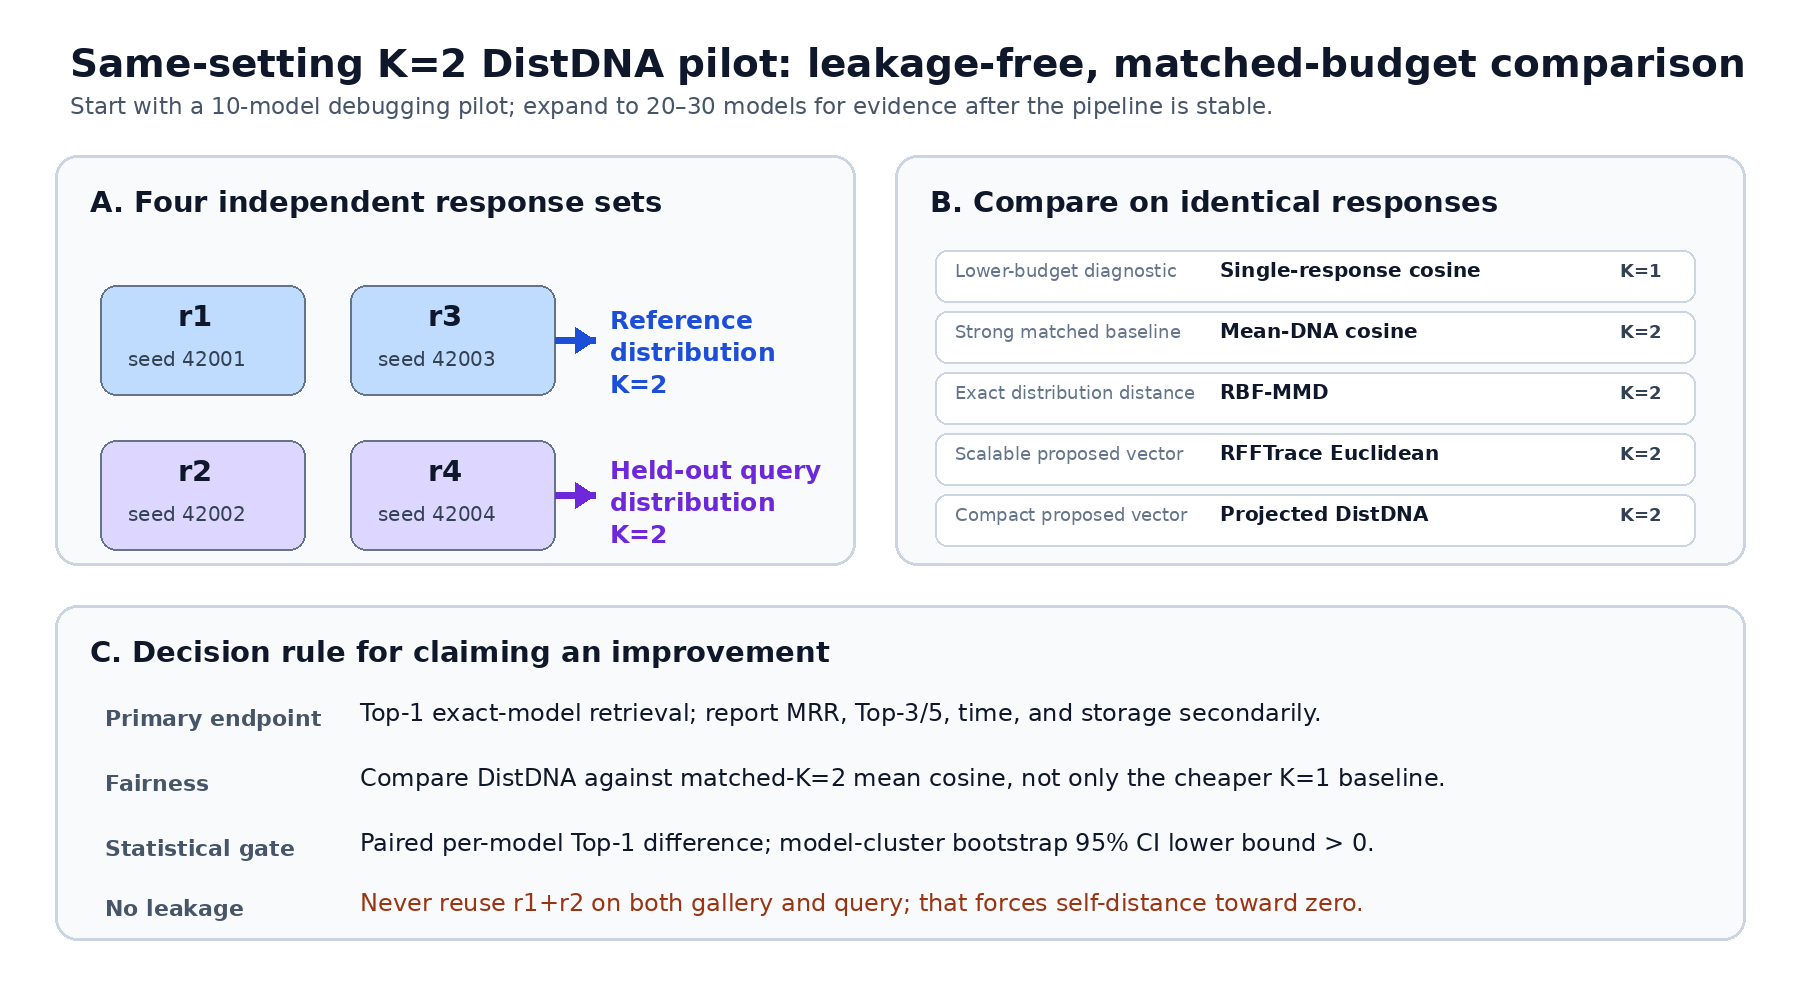
\includegraphics[width=\textwidth]{distdna_k2_pilot_design.png}
\caption{Leakage-free, matched-budget DistDNA pilot. Seeds 42001 and 42003
form the $K=2$ reference distribution; seeds 42002 and 42004 form the held-out
$K=2$ query distribution. Every $K=2$ method consumes the same responses.}
\label{fig:distdna-pilot}
\end{figure}

The ten-model cohort is fixed before DistDNA accuracy is inspected:

\begin{longtable}{r p{0.68\textwidth} r}
\caption{Proposed small-model pilot cohort.}\label{tab:pilot-cohort}\\
\toprule
No. & Model & Approx. scale \\
\midrule
\endfirsthead
\toprule
No. & Model & Approx. scale \\
\midrule
\endhead
1 & \nolinkurl{ibm-granite/granite-4.0-h-350m-base} & 0.35B \\
2 & \nolinkurl{EleutherAI/pythia-410m-seed1} & 0.41B \\
3 & \nolinkurl{EleutherAI/pythia-410m-seed2} & 0.41B \\
4 & \nolinkurl{EleutherAI/pythia-410m-seed3} & 0.41B \\
5 & \nolinkurl{unsloth/Qwen2.5-0.5B} & 0.50B \\
6 & \nolinkurl{unsloth/Qwen2.5-0.5B-Instruct} & 0.50B \\
7 & \nolinkurl{Ihor/Text2Graph-R1-Qwen2.5-0.5b} & 0.50B \\
8 & \nolinkurl{robowaifudev/megatron-gpt2-345m} & 0.35B \\
9 & \nolinkurl{state-spaces/mamba-370m-hf} & 0.37B \\
10 & \nolinkurl{unsloth/Qwen3-0.6B-Base} & 0.60B \\
\bottomrule
\end{longtable}

The repeated Pythia and Qwen families make the pilot less likely to saturate
than an arbitrary set of unrelated models. The parameter labels are advertised
model scales and must be checked against model metadata before launch.

\subsection{Fair comparison}

The pilot reports five retrieval methods:

\begin{enumerate}
  \item single-response cosine ($K=1$), as a lower-budget diagnostic;
  \item mean-DNA cosine ($K=2$), as the primary matched-budget baseline;
  \item exact RBF-MMD ($K=2$);
  \item RFFTrace ($K=2$); and
  \item compact projected DistDNA ($K=2$).
\end{enumerate}

The principal contrast is DistDNA minus mean-DNA cosine on the same query
models. Beating only the $K=1$ cosine baseline would not establish a
distributional advantage. Top-1 is primary; MRR, Top-3/5, runtime, and storage
are secondary. With ten query models, one corrected model changes Top-1 by ten
percentage points, so this pilot is suitable for debugging and effect direction
rather than a final confidence claim.

\section{Execution time and scale-out decision}

Historical successful primary artifacts required a median of 9.0 GPU-minutes
and a mean of 31.3 GPU-minutes per artifact; recognizable sub-0.8B models had a
median of 2.4 minutes but a long retry tail. Table~\ref{tab:timing} therefore
uses operational ranges rather than the median alone.

\begin{table}[htbp]
\centering
\caption{Estimated time after GPUs become available.}
\label{tab:timing}
\begin{tabularx}{\textwidth}{Xrr}
\toprule
Task & Four A100s & Eight A100s \\
\midrule
Ten-model, one-setting four-seed generation & 1--3 hours & below 2 hours \\
Checked first DistDNA comparison, including diagnostics & 4--8 hours & 4--8 hours \\
100 models, one setting, four seeds & 2--4 days & 1.5--3 days \\
100 models, all 12 stochastic settings, four seeds & 4--6 weeks & 2--3 weeks \\
\bottomrule
\end{tabularx}
\end{table}

At $T=0.7,p=1.0$, the four-seed target is 400 artifacts. Approximately 103
explicit 42001/42002 artifacts are already reusable, leaving roughly 297 new
artifacts. This one-setting extension should follow immediately after the
ten-model pilot passes its leakage and saturation checks. The all-setting
extension is a separate multi-week compute commitment and should be gated by
the pilot result.

Raw responses remain reusable when RFF dimension, kernel bandwidth, compact
projection, or the DistDNA vector is changed. Representation development can
therefore continue while the seed-explicit generation queue runs.

\section{Implementation and reproducibility}

The relevant implementation is:

\begin{itemize}
  \item distributional features and distances:
        \nolinkurl{src/llm_dna/distributional.py};
  \item matched-sample evaluator:
        \nolinkurl{scripts/run_rfftrace_experiment.py};
  \item optional SVM evaluator:
        \nolinkurl{scripts/evaluate_rfftrace_svm.py};
  \item live recovery and DistDNA design figures:
        \nolinkurl{scripts/plot_primary_status_and_distdna_design.py}; and
  \item temperature/top-$p$ and bounded-surface analysis:
        \nolinkurl{scripts/analyze_primary_decoding_surface.py}.
\end{itemize}

The new surface data are saved next to the figures as
\nolinkurl{primary_decoding_surface.csv},
\nolinkurl{primary_bounded_surface.csv}, and
\nolinkurl{primary_decoding_analysis.json}. Re-running the analysis while
recovery is active may change the strict cohort and reported values. The final
report must therefore regenerate all counts and accuracy figures after the
recovery process exits.

\end{document}
